\subsection{C6 -- Galactic orbital native window}\label{app:c6}
\paragraph{Native question.} Does the cited long-window galactic trace carry the predicted support mass, residual burden, cadence witness, drift witness, and effective progress-rate profile?
\paragraph{Native readout.}
\begin{itemize}
\item cited galactic window $\omega_{\mathrm{gal}}$
\item structural key \texttt{tetron:4:4:8}
\item frame count / $T_{\mathrm{eval}}=5000$ bip
\item weighting policy $w(\kappa)\equiv 1$
\item native radial grid
\end{itemize}
\paragraph{Native operator chain.}
\[
b(\kappa)\to H_B\to B^*\to \Lambda_b\to R_{\mathrm{rest}}\to \text{cadence witness},\ \text{drift witness},\ v(\omega).
\]
\paragraph{Native output row.}
\begin{center}
\small
\begin{tabular}{lcccccc}
\toprule
Row & Key & $B^*$ & $\Lambda_b$ & $R_{\mathrm{rest}}$ [trit/bip] & Cadence spectrum [cyc/bip] & Drift \\
\midrule
C6.A & tetron:4:4:8 & 137 & 8 & 0.0123 & $\{1/4,3/8\}$ & plateau \\
\bottomrule
\end{tabular}
\end{center}
\paragraph{Temporal Conversion Block.} Temporal conversion is a normal chain-rule expansion on the cited native row. At the current witness radius of $24$ kpc, the available speed witnesses are
\[
v_{\mathrm{classical}}=63.50852961085884\ \text{km/s},\qquad
v_{\mathrm{temporal}}=220.0\ \text{km/s},\qquad
v_{\mathrm{flat}}=220.0\ \text{km/s}.
\]
\paragraph{Native figure witness.}
\begin{center}
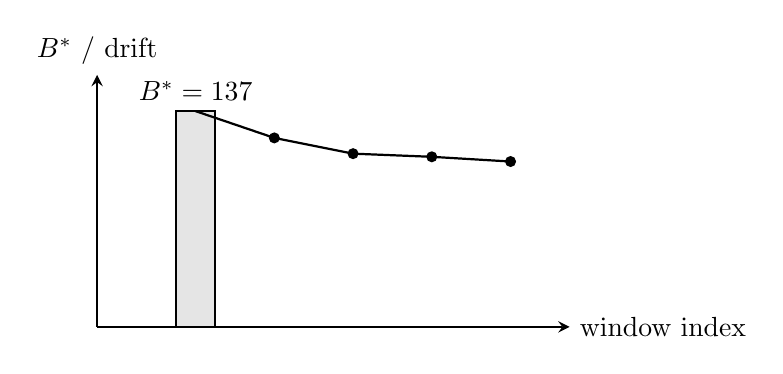
\begin{tikzpicture}[x=1.0cm,y=0.02cm,>=stealth,thick]
\draw[->] (0,0) -- (6,0) node[right] {window index};
\draw[->] (0,0) -- (0,160) node[above] {$B^*$ / drift};
\draw[fill=gray!20] (1,0) rectangle (1.5,137);
\draw (1.25,137)--(2.25,120)--(3.25,110)--(4.25,108)--(5.25,105);
\foreach \x/\y in {2.25/120,3.25/110,4.25/108,5.25/105}{\fill (\x,\y) circle (2pt);} 
\node[above] at (1.25,137) {$B^*=137$};
\end{tikzpicture}
\end{center}
\paragraph{Hook / Evidence.} Use the cited long-window drift and support hooks.
